\chapter{Expectations (Discrete)}
\label{chapter:ExpectationsDiscrete}

The PMF of random variable $X$ provides a complete characterization of the  random variable by specifying the probability of every possible outcome of $X$.
This description is, in general, very useful.
However, it is sometimes desirable to summarize the information contained in the PMF of a random variable to a few parameters.
This can be achieved using the concept of expectations.

Consider a discrete random variable $X$ with PMF $p_X$, and let $g$ be a real-value function on the range of $X$.
The \emph{expected value} of $g(X)$ is defined by
\begin{equation} \label{equation:Expectation}
\Expect \left[ g(X) \right]
= \sum_{x \in X(\Omega)} g(x) p_X (x) .
\end{equation}
It is important to realize that there exist random variables and functions for which the above sum does not converge.
In such cases, we simply say that the expected value of $g(X)$ does not exist.

\begin{example}
Let $g(x) = c$ be a constant, then the expectation of $g(X) = c$ is equal to
\begin{equation*}
\Expect \left[ c \right]
= \sum_{x \in X(\Omega)} c p_X (x)
= c \sum_{x \in X(\Omega)} p_X (x)
= c,
\end{equation*}
where the last inequality follows from the normalization axiom of probability laws.
We conclude that the expectation of a constant is the constant itself.
\end{example}

We introduced in section~\ref{subsection:FunctionDiscreteRV} functions of random variables.
Suppose that we create a new random variable $Y$ by applying a real-valued function $g$ to $X$,
\begin{equation*}
Y = g(X) .
\end{equation*}
We can compute the expectation of $Y$ using two different formula.
First, we can employ \eqref{equation:Expectation} directly to $Y$,
\begin{equation*}
\Expect [Y] = \sum_{y \in g(X(\Omega))} y p_Y(y),
\end{equation*}
where $p_Y (y)$ is given by \eqref{equation:FunctionPMF}.
Alternatively, we also have
\begin{equation*}
\Expect [Y] = \Expect [g(X)] = \sum_{x \in X(\Omega)} g(x) p_X(x) .
\end{equation*}
To verify that these formula are consistent, we proceed as follows
\begin{equation*}
\begin{split}
\Expect [Y] &= \sum_{y \in g(X(\Omega))} y p_Y(y) \\
&= \sum_{y \in g(X(\Omega))} y
\sum_{\{x \in X(\Omega) | g(x) = y\}} p_X(x) \\
&= \sum_{y \in g(X(\Omega))}
\sum_{\{x \in X(\Omega) | g(x) = y\}} y p_X(x) \\
&= \sum_{y \in g(X(\Omega))}
\sum_{\{x \in X(\Omega) | g(x) = y\}} g(x) p_X(x) \\
&= \sum_{x \in X(\Omega)} g(x) p_X(x)
= \Expect [g(X)].
\end{split}
\end{equation*}
Indeed these two methods of computing the expected value of $Y$ are equivalent.


\section{The Mean}

The simplest non-trivial expectation is called the \emph{mean}.
For random variable $X$, the mean is simply the expected value of $X$ itself.
It is represented by $\Expect [X]$ and, according to \eqref{equation:Expectation}, it is given by
\begin{equation*}
\Expect [X] = \sum_{x \in X(\Omega)} x p_X (x) .
\end{equation*}

\begin{example}
Let $X$ be a geometric random variable with
\begin{equation*}
p_X (k) = (1-p)^{k-1} p, \quad k = 1, 2, \ldots
\end{equation*}
The mean of this random variable is
\begin{equation*}
\begin{split}
\Expect [X] &= \sum_{k=1}^{\infty} k (1-p)^{k-1} p
= p \sum_{k=1}^{\infty} k (1-p)^{k-1}
= \frac{1}{p} .
\end{split}
\end{equation*}
\end{example}

\begin{example}
Let $X$ be a binomial random variable with
\begin{equation*}
p_X (k) = \binom{n}{k} p^k (1-p)^{n-k} ,
\end{equation*}
where $k = 0, 1, \ldots, n$.
The mean of this binomial random variable is computed as
\begin{equation*}
\begin{split}
\Expect [X] &= \sum_{k=0}^n k \binom{n}{k} p^k (1-p)^{n-k} \\
&= \sum_{k=1}^n \frac{n!}{(k-1)!(n-k)!} p^k (1-p)^{n-k} \\
&= \sum_{l=0}^{n-1} \frac{n!}{l!(n-1-l)!} p^{l+1} (1-p)^{n-l-1} \\
&= n p \sum_{l=0}^{n-1} \binom{n-1}{l} p^{l} (1-p)^{n-1-l}
= n p .
\end{split}
\end{equation*}
\end{example}

It may be insightful to relate the mean of a random variable to classical mechanics.
Let $X$ be a random variable and suppose that, for every $x \in X(\Omega)$, we place a stone of mass $p_X(x)$ at position $x$ along the real axis.
The mean of random variable $X$ coincides with the center of mass of the particles.

\begin{example}
Let $X$ be a Bernoulli random variable such that
\begin{equation*}
p_X (x) = \left\{ \begin{array}{ll}
0.25, & \text{if }x = 0 \\
0.75, & \text{if }x = 1.
\end{array} \right.
\end{equation*}
The mean of $X$ is given by
\begin{equation*}
\Expect [X] = 0 \times 0.25 + 1 \times 0.75 = 0.75 .
\end{equation*}
Consider a two-particle system with masses $m_1 = 0.25$ and $m_2 = 0.75$.
In the coordinate system illustrated below, the particles are located at $r_1 = 0$ and $r_2 = 1$.
Their center of mass is given by
\begin{equation*}
R = \frac{ m_1 r_1 + m_2 r_2 }{ m_1 + m_2 } = 0.75 .
\end{equation*}
The center of mass coincides with the mean of $X$.

\begin{figure}[ht]
\begin{center}
\includegraphics[height=1.8cm]{Figures/5Chapter/mass}
\end{center}
\caption{The center of mass on the figure is indicated by the tip of the arrow.}
\end{figure}
\end{example}

Suppose $X$ is a random variable with finite mean.
Let $Y$ be the affine function of $X$ given by
\begin{equation*}
Y = aX + b,
\end{equation*}
where $a$ and $b$ are fixed real numbers.
The mean of random variable $Y$ is given by
\begin{equation*}
\Expect [Y] = a \Expect [X] + b.
\end{equation*}
We can compute the mean of $Y$ using \eqref{equation:Expectation}.
It is equal to
\begin{equation*}
\begin{split}
\Expect [Y] &= \sum_{x \in X(\Omega)} (ax + b) p_X(x) \\
&= a \sum_{x \in X(\Omega)} x p_X(x) + b \sum_{x \in X(\Omega)} p_X(x) \\
&= a \Expect [X] + b.
\end{split}
\end{equation*}

It is not much harder to show that the expectation is a linear operator.
Suppose that $g$ and $h$ are two real-valued functions such that $\Expect [g(X)]$ and $\Expect [h(X)]$ exist.
We can compute the expectation of $a g(X) + h(X)$ as
\begin{equation*}
\begin{split}
\Expect [ a g(X) + h(X) ] &= \sum_{x \in X(\Omega)} (a g(x) + h(x)) p_X(x) \\
&= a \sum_{x \in X(\Omega)} g(x) p_X(x) + \sum_{x \in X(\Omega)} h(x) p_X(x) \\
&= a \Expect [g(X)] + \Expect [h(X)] .
\end{split}
\end{equation*}
That is, the expectation is both additive and homogeneous.


\section{The Variance}

The second most common descriptive quantity associated wth a random variable $X$ is its \emph{variance}, which we denote by $\Var (X)$.
It is defined by
\begin{equation} \label{equation:Variance}
\Var (X) = \Expect \left[ \left( X - \Expect [X] \right)^2 \right] .
\end{equation}
The variance is always nonnegative.
It provides a measure of the dispersion of $X$ around its mean.
For discrete random variables, it can be computed explicitly as
\begin{equation*}
\Var (X) = \sum_{x \in X(\Omega)} \left( X - \Expect [X] \right)^2 p_X (x) .
\end{equation*}
The square root of the variance is referred to as the \emph{standard deviation} of $X$, and it is denoted by $\sigma_X$.

\begin{example}
Let $X$ be a Poisson random variable with parameter $\lambda$.
The mean of $X$ is given by
\begin{equation*}
\Expect [X] = \sum_{k=0}^{\infty} k \frac{\lambda^k}{k!} e^{- \lambda}
= \sum_{k=1}^{\infty} \frac{\lambda^k}{(k-1)!} e^{- \lambda}
= \lambda \sum_{l=0}^{\infty} \frac{\lambda^l}{l!} e^{- \lambda}
= \lambda .
\end{equation*}
The variance of $X$ can be calculated as
\begin{equation*} \label{equation:VarianceExplicit}
\begin{split}
\Var (X) &= \sum_{k=0}^{\infty} \left( k - \lambda \right)^2
\frac{\lambda^k}{k!} e^{- \lambda} \\
&= \sum_{k=0}^{\infty} \left(\lambda^2 - 2 k \lambda + k + k(k-1) \right)
\frac{\lambda^k}{k!} e^{- \lambda} \\
&= \lambda^2 - 2 \lambda^2 + \lambda +
\sum_{k=0}^{\infty} k(k-1) \frac{\lambda^k}{k!} e^{- \lambda} \\
&= \lambda - \lambda^2 +
\sum_{k=2}^{\infty} \frac{\lambda^k}{(k-2)!} e^{- \lambda} \\
&= \lambda - \lambda^2 +
\lambda^2 \sum_{l=0}^{\infty} \frac{\lambda^l}{l!} e^{- \lambda}
= \lambda .
\end{split}
\end{equation*}
Both the mean and the variance of a Poisson random variable with parameter $\lambda$ are equal to $\lambda$.
\end{example}

\begin{theorem}
Suppose $X$ is a random variable with finite mean and variance, and let $Y$ be the affine function of $X$ given by $Y = aX + b$, where $a$ and $b$ are constants.
The variance of $Y$ is given by
\begin{equation*}
\Expect [Y] = a \Expect [X] + b.
\end{equation*}
\end{theorem}
\begin{proof}
Consider \eqref{equation:VarianceExplicit} applied to $Y = aX + b$.
\begin{equation*}
\begin{split}
\Var(Y)
&= \sum_{x \in X(\Omega)} \left( ax + b - \Expect [aX + b] \right)^2 p_X(x) \\
&= \sum_{x \in X(\Omega)} \left( ax + b - a \Expect [X] - b \right)^2 p_X(x) \\
&= a^2 \sum_{x \in X(\Omega)} \left( x - \Expect [X] \right)^2 p_X(x)
= a^2 \Var(X) .
\end{split}
\end{equation*}
Clearly, the variance is not a linear operator.
\end{proof}


\section{Moments}

The \emph{moments} of a random variable $X$ are likewise important quantities used in summarizing the PMF of $X$.
The $n$th moment of random variable $X$ is defined by
\begin{equation*}
\Expect [X^n] = \sum_{x \in X(\Omega)} x^n p_X (x) .
\end{equation*}
The mean of a random variable is also its first moment.
The variance of the random variable $X$ can be defined in terms of its first two moments, $\Expect [X]$ and $\Expect [X^2]$.
This alternate formula is sometimes convenient for computation purposes.

\begin{theorem}
The variance of random variable $X$ can be expressed in terms of the moments of $X$,
\begin{equation*}
\Var (X) = \Expect \left[ X^2 \right] - \left( \Expect [X] \right)^2.
\end{equation*}
\end{theorem}
\begin{proof}
Suppose that the variance of $X$ is finite.
We can expand \eqref{equation:Variance} as
\begin{equation*}
\begin{split}
\Var (X) &= \sum_{x \in X(\Omega)} \left( x - \Expect [X] \right)^2 p_X (x) \\
&= \sum_{x \in X(\Omega)} \left( x^2 - 2 x \Expect [X] + \left( \Expect [X] \right)^2 \right) p_X (x) \\
&= \sum_{x \in X(\Omega)} x^2 p_X (x) - 2 \Expect [X] \sum_{x \in X(\Omega)} x p_X (x) + \left( \Expect [X] \right)^2 \sum_{x \in X(\Omega)} p_X (x) \\
&= \Expect \left[ X^2 \right] - \left( \Expect [X] \right)^2.
\end{split}
\end{equation*}
This alternate formula for the variance of $X$ is sometimes easier to compute.
\end{proof}

\begin{example}
Let $X$ be a discrete uniform random variable with PMF
\begin{equation*}
p_X (k) = \left\{ \begin{array}{ll}
1/n, & \text{if }k = 1, 2, \ldots, n \\
0, & \text{otherwise} .
\end{array} \right.
\end{equation*}
The mean of this uniform random variable is easily seen to equal
\begin{equation*}
\Expect [X] = \frac{n+1}{2} .
\end{equation*}
Its variance is obtained  as
\begin{equation*}
\begin{split}
\Var (X) &= \Expect [X^2] - \left( \Expect [X] \right)^2 \\
&= \sum_{k=1}^n \frac{k^2}{n} - \left( \frac{n+1}{2} \right)^2 \\
&= \frac{n(n+1)(2n+1)}{6} - \left( \frac{n+1}{2} \right)^2 \\
&= \frac{4 n^3 + 3 n^2 - 4 n -3}{12} .
\end{split}
\end{equation*}
\end{example}

